%-----------------------------------------------------------------------------
% Template for seminar 'Program Analysis' at TU Darmstadt.
%
% Adapted from template for sigplanconf LaTeX Class, which is a LaTeX 2e
% class file for SIGPLAN conference proceedings (by Paul C.
% Anagnostopoulos).
%
%-----------------------------------------------------------------------------


\documentclass[authoryear,preprint, twocolumn]{sigplanconf}

	
% A couple of packages that may be useful
\usepackage{amsmath}
\usepackage{amsfonts}
\usepackage{amssymb}
\usepackage{amsthm}
\usepackage{algorithm2e}
\usepackage{listings}
\usepackage{xcolor}
\usepackage{tikz}
\usepackage{booktabs}
\usepackage{subfigure}
\usepackage[english]{babel}
\usepackage{blindtext}

%Added for JavaScript syntax highlighting
\definecolor{purple}{rgb}{0.65, 0.12, 0.82}
\lstdefinelanguage{JavaScript}{
	keywords={break, case, catch, continue, debugger, default, delete, do, else, false, finally, for, function, if, in, instanceof, new, null, return, switch, this, throw, true, try, typeof, var, void, while, with},
	morecomment=[l]{//},
	morecomment=[s]{/*}{*/},
	morestring=[b]',
	morestring=[b]",
	ndkeywords={class, export, boolean, throw, implements, import, this},
	keywordstyle=\color{blue}\bfseries,
	ndkeywordstyle=\color{darkgray}\bfseries,
	identifierstyle=\color{black},
	commentstyle=\color{purple}\ttfamily,
	stringstyle=\color{red}\ttfamily,
	sensitive=true
}

\lstset{
	language=JavaScript,
	extendedchars=true,
	basicstyle=\footnotesize\ttfamily,
	showstringspaces=true,
	showspaces=false,
	numberstyle=\footnotesize,
	numbersep= 4pt,
	tabsize=4,
	breaklines=true,
	showtabs=false,
	captionpos=b,
	xleftmargin=\parindent
}
%end JavaScript syntax highlighting

\begin{document}

\special{papersize=a4}
\setlength{\pdfpageheight}{\paperheight}
\setlength{\pdfpagewidth}{\paperwidth}


\title{GUI Testing - Prospective \& Analysis}

\authorinfo{Pranay Sarkar}
{Fachbereich Informatik\\
		Technische Universit{\"a}t Darmstadt\\
		Hochschulstra{\ss}e 10 , 64289 Darmstadt\\
		Email: pranay.sarkar@stud.tu-darmstadt.de}
	{Matriculation Number: 2337328}
\maketitle

\begin{abstract}
Graphical User Interface \emph{(GUI)} testing is the method of testing an application via its GUI. The generic goal is to ensure that it meets the specifications by identifying the presence of defects in the software product. Normally this kind of testing is done by using different test cases. Generated test cases should try to cover all functionalities of the GUI. There are two ways to generate test cases: Manually and Randomly. GUI normally have huge search space which makes exhaustive iteration of all states almost impossible. So the general approach is to steer towards potential bugs or unexplored behaviors. It can be accomplished by a automated testing combined with approximate learning. Here, in this paper we will mainly discuss about 3 GUI testing techniques:
\begin{itemize}
	\item Artemis - framework for feedback directed automated testing of JavaScript applications.
	\item EventBreak - performance guided test generation process which analyze and identify slowdown pairs among events.
	\item SwiftHand - Automated approximate learning GUI testing of Android applications with minimal restart.
\end{itemize}

%Adding keywords (Pranay)
{\bf Keywords:} GUI Testing, Web Applications, Testing, Responsiveness, Test Generation, Android, Automata, Testing and Debugging
\end{abstract}




\section{Introduction}
\label{sec:introduction}

Modern GUI of web and Android applications in Smartphones, tablets depend on JavaScript and different event driven user interfaces. Applications for mobile devices are called 'Apps'
\newline There are mainly three different existing approaches to GUI testing:
\begin{itemize}
	\item Manual testing - It is based on a particular application, domain and the knowledge of tester.
	\item Capture and replay based - It involves capturing user action and replaying it while testing.
	\item Model based - It is dependent on user session execution and based on a specific GUI model. Those can be Event based models where events in GUI need to be executed at least once, State based models where all states in the GUI need to be executed at least once and Domain based model which depends on application domain and functionality.
\end{itemize}
Generally different GUI testing methods focus on - checking screen validations, verifying all navigations, checking usability conditions, verifying data integrity, object states, and all available date fields and numeric fiends in the GUI.
\newline But GUI testing introduces some new challenges. First challenge is faced while trying to cover all functionality in the system. The problem lies in te domain size of GUI and sequencing. Additionally, if the goal is to do regression testing, it becomes more difficult because GUI can have significant changes even if the  underlaying application does not change. For example, when a button or dialog or menu item changes its position or design, any GUI test which is following a certain path may fail. Second challenge is sequencing. Some GUI functionalities can be reached only after going through a particular sequence of previous events. If the number of dependent event is high, the amount of combination will become too large to do GUI testing with good code and branch coverage. For example, in \emph{LibreOffice Writer} (document editor), to change the font style and formatting user have to click on \emph{Format} then \emph{Styles and Formatting}, where Format drop-down menu have a total of 21 items and at last user has to focus on the newly opened window. It can be seen from this example that increasing the possible number of operations exponentially increases the sequencing problem.
\newline These two issues are the driving factor for adding some kind of feedback adaptive or performance guided or approximate learning based GUI testing algorithms. 
\newline Several research projects tried to solve these problem by using automated testing. \emph{Crawljax/Atusa project} does dynamic analysis of application state space and generates test case. Limitation is it may not be able to detect all relevant event handlers. \emph{Kudzu Project} adds random test generation in application's event space with symbolic execution in application's value space. But it relies on String and string operations which can be easily manipulated by JavaScript applications.
\newline The following three discussed algorithms addresses these problems and specifically tries to negate the two aforementioned challenges.
\newline \emph{Artemis} - a framework for feedback directed GUI testing, instantiates with different prioritization functions and input generators. It uses several realistic test generational algorithms - \emph{events}, \emph{const}, \emph{cov}, \emph{all}. %\cite{Artemis1}
\newline \emph{EventBreak} identifies and analyzes set of available events to identify pair of event handlers whose execution time can increase gradually with respect to time. It can happen when triggering one event increases execution time of other event. It gather data from performance history and compare it to the execution cost of current events to determine which events are responsible for system slowdown.
\newline \emph{SwiftHand} is a framework for generating sequence of inputs for testing Android apps. This algorithm uses machine learning models to learn model of testing app. It can use the learned model to generate different user inputs which tries to visit most unexplored states in the app. Model of testing app is completely adaptive to future changes and can be integrated with newly learned information from machine learning algorithm.
\begin{figure*}[!t]
	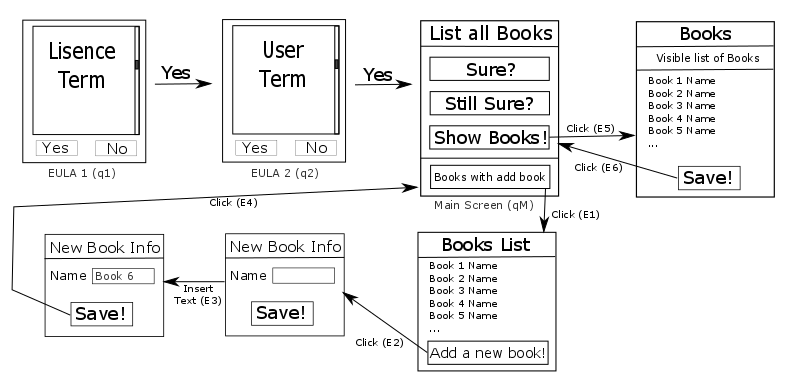
\includegraphics[width=\textwidth]{figures/ptaArchitecture0002}
	\caption[Block diagram for motivation example system]{\label{f:sysarchtect}Block diagram for motivation example system}
\end{figure*}

\newline The following program can be considered as a \emph{motivating example} from now on:
\newline Consider a virtual book store, which can be Android or browser based running using JavaScript. It shows list of all available books and have the capability to add new books to the available book list. User need to accept \emph{License terms} and \emph{User terms}, which comes in 2 separate pages before getting access to the book store. \emph{User terms} comes only after accepting (i.e. clicking \emph{Yes} button) in the \emph{License terms} page. Android version of the app allows us to use \emph{SwiftHand} algorithm on it.
\newline System block diagram: \emph{Figure 1}.

%\begin{figure*}[t]
%	
\includegraphics[width=\textwidth,height=4cm]{figures/SOLALogo}
%	\caption{Test image.}
%\end{figure*}

\newline Two most interesting parts of this programs are:
\newline If Button 1 \emph{(Sure?)} and Button2 \emph{(Still sure?)} are clicked then only clicking 'Show Books' button lists all books:

\begin{lstlisting}[caption=Code for activating Book Listing button for the first time,label=2,language=JavaScript]
var button1 = false;
var button2 = false;
document.getElementById("sure").onclick = function() {button1 = true; }
document.getElementById("still sure").onclick = function() {button2 = true; }

if(button1){
	if(button2){
		window.alert("BookList activated");
		document.getElementById("showBooks").onclick = booklist.show();
	}
}
\end{lstlisting}

\newline And this part of code for adding new books in the existing list of books:

\begin{lstlisting}[caption=Code for adding and validating new bok,label=2,language=JavaScript]
var bookelements = form.getElements('bookset')
	.concat(Array.form(from.elements));
//Iterating over all book list before adding
for (var i=0; i <bookelements.length; i++){
	if(this.validate(elements[i]) == false){
		validity = false;
	}
}
\end{lstlisting}

\newline Remaining part of the paper is organized as follows. In section 2, Artemis, the feedback direct GUI testing algorithm is described. Section 3 consist of EventBreak, used for responsiveness testing and to find \emph{slowdown pairs}. Section 4 have details of last discussed algorithm. SwiftHand, a model interface based testing for Android \emph{apps} with minimum amount of restart. Comparison of performance and how these algorithm works on the above mentioned motivation example, are discussed in Section 5. 


%\section{Artemis - Framework for Automated Testing of JavaScript web applications}
\section{Artemis - Feedback Directed GUI Testing}
\label{sec:artemis}
There is very little tool support for testing JavaScript programs compared to other languages such as C\#, Java. Test cases are usually generated manually using Unit test tools such as Selenium, Sahi and Watir. JavaScript programs are written in event-driven style, which produces very large number of possible combinational states. This presents a huge problem for obtaining good test coverage by only using manual testing.
\newline Artemis is a framework for testing JavaScript web applications which combines automated testing with feedbacks from earlier test cases. It gives high code coverage while discovering the errors.
\newline Artemis takes event driven execution model of JavaScript and interaction with Document Object Model (DOM) of web pages. Parameters of the framework are: (a) an \emph{execution unit} $\mathcal{E}$ for modeling the browser and server, (b) an \emph{input generator} $\mathcal{G}$ for producing new input sequence, (c) a \emph{prioritizer} $\mathcal{P}$ for guiding application's state space exploration. These parameters can be instantiated differently and that will make various forms of feedback-directed testing possible(e.g. Randoop).
\newline Artemis starts with events which are randomly selected from the list of available events obverses the event and gathers feedback from the execution. Feedback can be gathered from available events, source code of handlers attached to events, memory locations where read and write happens, branch coverage. It can be used to generate additional test inputs, which will gradually steers towards particular interesting behavior.
\newline While loading a web page, browser parses HTML contents into a DOM structure and executes JavaScript code. Event handlers including those which may be triggered later are registered at that point of time. JavaScript event is a unit record where all possible values for parameter are valid. Event consist of \emph{(i)} an event parameter map, \emph{(ii)} a form state map, \emph{(iii)} an environment that holds user controlled constituents of browser state. Test input consists of \emph{(i)} URL to a web page, \emph{(ii)} entry state describing state of server, \emph{(iii)} sequence of aforementioned structured events.
\newline Artemis starts with URL of main test window. In our case, \emph{License terms}. While executing test inputs to the URL, other windows or frames may be created (e.g. User terms). Execution unit in Artemis manages them as a single combined JavaScript DOM structure. 
\newline Prioritization function $\mathcal{P}$.\emph{priority(c)} for a input c = (u,S,$s_1$,...$s_n$) is defined as the product of all prioritization functions, where ei is the set of event handlers. Algorithm begin by assigning same priority to all events (i.e. $P_0$(c)  = 1). As the algorithm goes on running sequence of event handlers having almost 100\% of code coverage is useless compared to executing sequences whose coverage is comparatively lower. So the final coverage function is defined as:
$P_1$(c) = 1- cov($e_1$) x ... x cov($e_n$)
where cov(s) contains information about event handlers as well as functions invoked by that event handler.
\newline Prioritization can also be based on read/write sets, where Artemis keeps track  of memory location read or written by each event handler. Higher priority is given to te sequences of events where values written by some event handlers are read by subsequence handler. In the given example if we consider \emph{List All Books page}, values of button1 and button2 are changed after clicking which are read by \emph{button3} (i.e. Show Books!) activating the list of books.
\newline Input generators have two alternative implementations. Default input generation strategy \emph{G0} is to choose a reasonable default value for all events. Another method is to dynamically collect constants where execution unit $\mathcal{E}$ is extended for tracking constants. Each event handler maintains a set of constants which are encountered while executing the event in \emph{const(e)}.

\begin{table}[ht]
	\centering
	\begin{tabular}{lll}
		\hline
		\textbf{} & \textbf{Prioritization function} & \textbf{Input Generator}\\
		\hline
		events	& $P_0$	& $G_0$\\
		\hline
		const	& $P_0$	& $G_1$\\
		\hline
		cov		& $P_0*P1$	& $G_1$\\
		\hline
		all.	& $P_0*P1*P2$	& $G1$\\
	\end{tabular}
	\caption[Test Generation algorithms]{\label{t:testGenerators}Test Generation algorithms.}
\end{table}

\newline Artemis considers all four feedback directed test generation algorithm - \emph{events}, \emph{const}, \emph{cov}, \emph{all}. These are constructed by initializing the framework with different prioritization functions and the above mentioned input generators. In the example's main page if we consider coverage guided prioritization functions and assume button1 (i.e. Sure?) is clicked and after that button3 (i.e. Show Books!) are clicked then initial coverages are: cov(button1) = 1, cov(button2) = 0, cov(button3) =2/5.
\newline Next possible event sequence would be: 
\begin{itemize}
	\item (button1, button3, button2) 
	\item (button1, button3, button1)
	\item (button1, button3, button3) 
\end{itemize}
and their priority $\mathcal{P}$ will be 1, 3/5 and 21/25 respectively. As the first mentioned sequence have highest priority, if that is executed, it will give highest code coverage.


%\section{EventBreak - Analyzing responsiveness of UI by Performance Guided Test generation}
\section{EventBreak - Responsiveness Testing for GUI}
\label{sec:eventbreak}
Most of the web applications have event driven interface which generally have a dedicated single thread for processing event handlers. JavaScript have event dispatcher which takes event handlers from a queue dispatching them to execution thread. Here the problem is browser does not react to user input while the event handler is executing. Because of this, if an event handler runs for too long, application is considered as unresponsive. 
\newline It is very hard to find unresponsiveness problem because application becomes unresponsive only after executing specific sequence of events. Manual testing is more concerned with code coverage whereas here the need is to test a specific area of a code for long enough to find the  reason for unresponsiveness.
\newline EventBreak, a performance guided test generation framework which creates sequence of user events and identifies pair of events, which can make the application unresponsive as one event increases the execution time of other event. This pair of events are called \emph{Slowdown pair}. EventBreak can be considered as cost plot set which shows tat execution time of one event changes because of triggering another event.
\newline EventBreak can be used in two kind of approaches. \emph{(i)} As a fully automated testing: it starts by randomly exploring the application for potential unresponsiveness problem, targeting exploration towards discovered potential slowdown pairs. \emph{(ii)} Leveraging existing test or use traces: It uses already available information about potential slowdown pairs and analyzes them in more details.
\newline EventBreak have \emph{two phases} to discover responsiveness problems. 
\newline \textbf{First phase:} It passively obverses and records the associated execution cost of each triggered event. It is done while loading the website and querying for currently enabled events. Then algorithm randomly picks an event from the list of enabled events. If any \emph{'back to referrer'} event is available test generator goes back to a referred with probability of ($\beta$) and then it can pick up other events with the probability of (1-$\beta$). Test generator then executes the event \emph{e} and measures then related cost \emph{c(e)} and append the cost to event-cost history (\emph{h}), which is sequence of pairs (e0,c0),.... (en,cn) where 
\begin{itemize}
	\item \emph{$e_i$} is an event,
	\item \emph{$c_i$} is cost associated while handling or executing the event = \emph{$c_{(ei)}$}
	\item \emph{$e_0$} is the initially triggered event
	\item \emph{$e_{(i+1)}$} is the event triggered in the reached state by \emph{$e_i$}
\end{itemize}

\newline It can also build upon existing testing efforts and using already obtained trace from a test suite or from recorded traces from  real users. In an alternative approach to random exploration of application, EventBreak can incorporate manual testing method. Then it records the events and associated costs triggered by the user. Cost is counted as the number of executed conditionals (e.g. \textmd{if, while, for, do while, for in}) during execution. For example, when we consider the motivating example's \emph{List All Books} page, let's assume that there is a statement \emph{count++} and we increase the counter at each function entry assuming that function dispatch is conditional. In \emph{Figure 2} related event-cost history is shown. It should be noted that in reality cost values can be higher as many event handlers can execute hundreds of conditions.

\begin{figure}[ht]
	\centering
	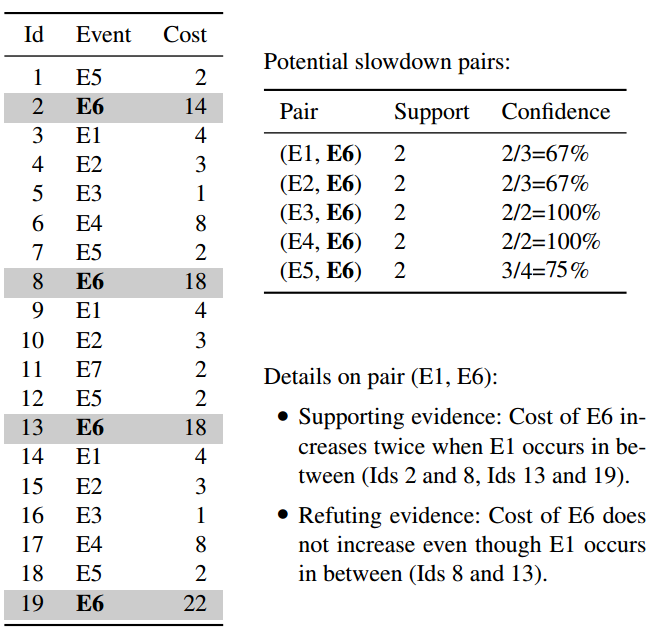
\includegraphics[width=1.0\linewidth]{figures/eventbreak1}
	\caption[Example of event-cost history and inference of potential slowdown pairs]{\label{f:approxappmodel}Example of event-cost history and inference of potential slowdown pairs [7]}
\end{figure}

\newline \textbf{Second phase:} It does detailed exploration of potential slowdown pairs on the hypothesis that the given pair is indeed a slowdown pair. Exploration is done by generating sequence of input events triggering both events in slowdown pair. For a slowdown pair (\emph{e cause, e effect}), EventBreak analyzes how cost of \emph{e\textsuperscript{effect}} changes with time. The algorithm mentioned in \emph{EventBreak} paper, for a candidate slowdown pair s, makes 2 maps: \emph{AllEvidences} is number of evidence related to s and \emph{SuppEvidence} is number of pieces of evidence to support the hypothesis that s is slowdown pair. Algorithm have a minimum confidence level and the current confidence level for the slowdown pair is measured by:\begin{center}
	 $\dfrac{SuppEvidence(s)}{AllEvidence(s)}$\begin{center}	
	 \end{center}
\end{center}

\newline For targeted exploration of \emph{SlowdownPairs}, EventBreak tries to confirm whether the potential slowdown pair can indeed increase the cost of handling event e\textsuperscript{effect}. But one major problem is application needs to in the state where the event is available to trigger that particular event.

\begin{figure}[ht]
	\centering
	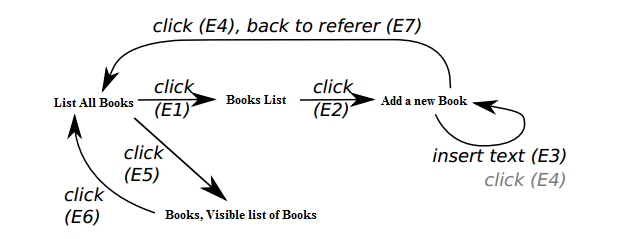
\includegraphics[width=1.0\linewidth]{figures/eventbreak2}
	\caption[Approximate Application model for List All Books page]{\label{f:eventcosthistory}Approximate Application model for List All Books page}
\end{figure}

\newline When triggering one event immediately after another event is not possible, EventBreak uses an inferred finite state model of the application. That application model can be non-deterministic finite state machine that had model states, and it can abstract application states and events, which are transition between the  states. EventBreak applies algorithm for passive automata learning to sequence events in event-cost history and thereby obtaining approximate model. Here in our motivation example, Approximate learning model for $List All Books page$ is described in \emph{Figure 3}. It should be mentioned that, this model can suffer from over-approximation or under-approximation.


%\section{SwiftHand - Guided GUI Testing for android apps with minimal restart and Approximate learning}
\section{Swifthand - Model interface based testing}
\label{sec:swifthand}

Mobile platforms like Smartphones and tablets are operated on specialized applications called \emph{apps}. Widely used GUI testing tools for the apps normally involves manually making scripting input sequence in python (e.g. MonkeyRunner [2]) or randomly generating sequence without taking into account position of actual controls (e.g. Monkey [3]). To avoid these problems, \emph{SwiftHand} mainly focus on learning and exploring abstraction model of GUI app with the goal of achieving code coverage quickly. But learning algorithms need to restart the app to go back to initial state and explore additional reachable states from it. It creates a practical problem with Android apps as restart means removing and reinstalling the app, which is complex and also takes more time, which normally takes 30 seconds. It is also noticed that by the use of 'back' or 'home' button most other interface screens can be reached. 
\newline Since this cost of restart is too high \emph{SwiftHand} tries to minimize the number of restarts by using learned model to choose user inputs which will take the app to previous states. While triggering newly generated user inputs SwiftHand expands and refines the existing model.
\newline In our motivating example, first two windows (i.e. \emph{License term} and \emph{User term} ) have scroll bar. We are considering License term as \emph{$q_1$}, User term as \emph{$q_2$} and Main window - List of Books as \emph{$q_M$}

\begin{figure}[ht]
	\centering
	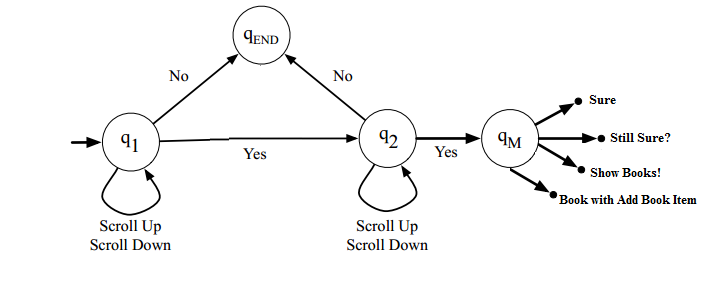
\includegraphics[width=1.0\linewidth]{figures/swifthand1}
	\caption[Partial model for motivation example Android app version]{\label{f:partialmodelandroid}Partial model for motivation example Android app version}
\end{figure}

\newline As testing interface \emph{SwiftHand} sends a user input to app and can wait for 5 seconds for the app to be stable. While making user interface model, SwiftHand  compares user interfaces by checking whether they have similar set of user inputs or not.
\newline \emph{SwiftHand} started by launching the app and waiting for the app to be stable. This state can be considered as \emph{initial app state}. Different \emph{Model States} can be computed based on the set of enabled user inputs along with the bounded screen co-ordinates where thy are enabled. If the model state have minimum one outgoing unexplored transition that is called \emph{frontier model-state}. If this state is not found, SwiftHand restarts the app. If a new app-state is found, SwiftHand adds the transition to it in the model. If the new app-state is equivalent, then states are merged together. After merging if it can not find any app-state visited earlier, it means merging is aggressive and it runs a passive learning algorithm using already executed traces. It should be noted that the main goal is not to learn the exact model but to achieve quick coverage.

\begin{figure}[ht]
	\centering
	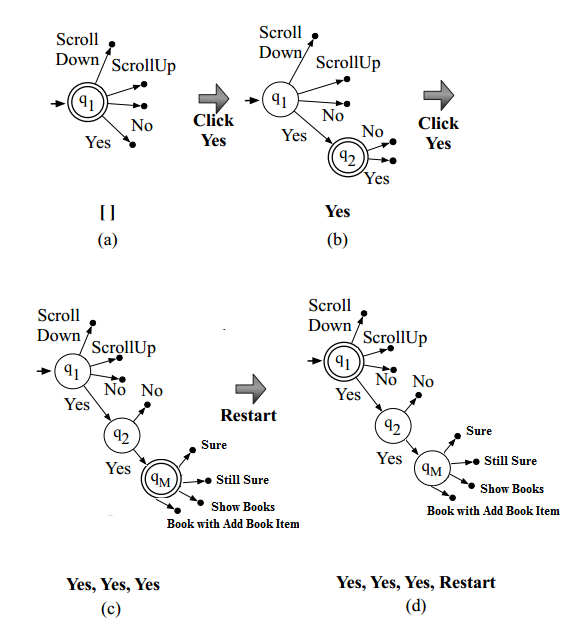
\includegraphics[width=1.0\linewidth]{figures/swifthand2}
	\caption[Progress of Guided learning testing. Circle with double line denotes current.state model, and with single line denotes state]{\label{f:guidedtestingmodel}Progress of Guided learning testing. Circle with double line denotes current.state model, and with single line denotes state}
\end{figure}

\newline Progress of SwiftHand in the motivating example is explained in \emph{Figure 5}, which involved 3 iterations. We may restart the app while executing SwiftHand but that will not affect the given result.
\begin{itemize}
	\item \emph{Initialization:} After launching and waiting for the app to be stable the reached state is initial state. It have 4 enabled input set \{\textbf{Yes}, \textbf{No}, \textbf{Scroll-up}, \textbf{Scroll-down}\}. Abstraction of the state $q_1$ is done as model-state in \emph{Figure 5(a)}.

	\item \emph{First Iteration:} SwiftHand finds the state q1 as \emph{frontier state} and choose to execute transition for \textbf{Yes}. Resulting set have different set of enabled inputs compared to the initial state. So the algorithm adds a new model-state $q_2$ to the learned model. Modified model can be seen in \emph{Figure 5(b)}.

	\item \emph{Second Iteration:} App is not in an app-state where corresponding model-state is $q_2$. Although both $q_1$ and $q_2$ have unexplored outgoing transitions, and our main goal is to minimize app restart, now we can only pick a transition from q2 as present model have no transition in it that can go back to $q_1$ form $q_2$ without restart. So \emph{SwiftHand} chooses the next input as \textbf{Yes}. Resulting set have different set of enabled inputs (i.e. \textbf{Sure}, \textbf{Still Sure?}, \textbf{Show Books!}, \textbf{Books with Add Book}) and algorithm adds a new model-state $q_M$ to the already learned model. Modified model is shown in \emph{Figure 5(c)}.

	\item \emph{Third Iteration:} SwiftHand does a forced restart of the app when it has already executed predefined number of user inputs from the app initial state. Assuming that restart happens in the third iteration, and after restart $q_1$ becomes the current-state, again. Assuming that \emph{SwiftHand} picks \textbf{Scroll-up} from $q_1$ it reaches a state which already have same set of enabled inputs \{\textbf{Yes}, \textbf{No}, \textbf{Scroll-up}, \textbf{Scroll-down}\}. So, that new model-state is merged with $q_1$ and the current-state in the learned model.
\end{itemize}

\newline After first three iterations \emph{SwiftHand} will execute 3 restarts and 8 more user inputs, in worse case, to learn the partial model figure shown in \emph{Figure 4}. Restarts are needed to know te terminal state $End$. It is observed that in the real-world benchmarks SwiftHand will spend 10\% of total time in restarting. 
\newline Some of the notable features of \emph{SwiftHand} are how the algorithm detects app termination an end of a state transition.
\begin{itemize}
	\item \textbf{App Termination Detection:} Android app consists of set of activities. Each activity implements single application screen and a set of functionality. All activities are stopped when app is terminated. So to track app termination tracking all activities of the app is enough. This can be done by periodically checking the app by an observer thread. \emph{SwiftHand} uses Android Activity Life-cycle based state tracking mechanism. Activity life-cycle  have six states: \emph{created}, \emph{started}, \emph{resumed}, \emph{paused}, \emph{stopped} and \emph{destroyed}. At the point of changing activity state, Android triggers fixed set f event handlers in a predefined order. \emph{SwiftHand} uses finite state machine to track current activity. A separate state machine is used for each instance of activity class.
	
	\item \textbf{End of a State Transition Detection:} During state transition number of event handlers are executed and screen content is also modified. So, after sending any transition command, \emph{SwiftHand} must wait for all event handlers and to complete their execution and screen content to finish all the modification. But a single event can trigger multiple event handlers.It is observed during the other experiments that 200 milliseconds and 1000 milliseconds are enough for real phones and emulators, respectively. \emph{SwiftHand} checks for stabilization of screen content by periodically checking for coordinate and size information of GUI components,before it trigger events through \textsf{chimpchat}. If there is no change fr a while, it can be concluded that the screen is stable. In other experiments it is observed that 1100 milliseconds and 1800 milliseconds are enough for real phones and emulators respectively.
\end{itemize}

\newline SwiftHand uses a modified variant of Lambeau et al's state merging algorithm. It uses $\lambda$ function or set of enabled transitions to avoid illegal merging, and the modified algorithm have no notion if negative examples. SwiftHand is implemented using Java and Scala.


\section{Comparison of three algorithms}
\label{sec:comparison}

Here motivation example is designed in such a way that all three algorithms are applied, but not in the whole example, but each of them are applied in some specific pages/activities. \textbf{Artemis} is applied in \emph{List All Books} page only, \textbf{EventBreak} is applied to \emph{List All Books}, \emph{Books List}, \emph{New Book Info}, \emph{Visible List of Books} pages, and \textbf{SwiftHand} is applied to \emph{License Term}, \emph{User Term} and \emph{List All Books} pages. It is done mainly to come up with an idea about how to integrate all 3 algorithms in one place. It is also assumed that we are working with two different version of same application: 
\begin{itemize}
	\item Web Version (JavaScript based, mostly)
	\item Android Version 
\end{itemize}
Android version is there specifically to test SwiftHand, which is meant for application running Android 4.1 or higher.

\newline Here we have applied \emph{Artemis}, and assumed that 2 buttons in the main screen is already clicked. Algorithm generated next possible sequence of events and applied prioritizer in it. That resulted in maximum code coverage for the given example page. Read-write set based prioritization is also considered there when the program reads the variables $button1$ and $button2$ and checks if they are $false$ or not before executing the functionality of \emph{Show Books!} button. So, these two write function of $button1$ and $button2$ are given higher priority as per the algorithm which states that \textit{Prioritize sequences where some handlers write values read by a subsequent handler} %\cite{gui-slides}.
In the main \emph{EventBreak} paper it is mentioned that basic algorithm \emph{events} produces 69\% of coverage and if the test generation is coverage information and read-write set directed, as it is done in \emph{cov} and \emph{all} algorithm, even better code coverage (i.e. 72\%) can be achieved. It satisfies the initial goal of achieving high code coverage.
\newline Testing algorithms are mostly concerned with gaining highest possible code coverage. But \emph{EventBreak} mainly concerns itself with looking into the details of specific part of code (i.e. \emph{Slowdown Pair}). This is a problem that is faced while comparing performance of \emph{EventBreak}, which will be obviously, low, all the time.  Another one of the main issues is to find out the state from where the event e\textsuperscript{effect} can be triggered. Searching for specific state in huge state space consumes lot of time. Another problem of EventBreak lies in approximation model. Shortest event sequence to target application may not be feasible because of over-approximation, and in the same way, approximate model may not include some sequence leaning from current state to target event due to under-approximation. Another problem with \emph{EventBreak} is, its overall effectiveness depends heavily on the initially exposed potential slowdown pairs. But the advantage of \emph{EventBreak} is, after analyzing the generated plots, understanding the reason of slowdown in performance becomes easier. \emph{EventBreak} can build on other drivers (i.e. more sophisticated automated test generation approaches) [7] during the first phase. It can also take the advantage of existing testing suites and help turning them into responsiveness tests via amplifying the initial execution. 
\newline In this example, passive re-learning technique can not be shown but it can done in \emph{SwiftHand}. The main goal of the algorithm is to achieve high branch converge, quickly. Main advantage of \emph{SwiftHand}, unlike other learning algorithms, is it searches for ways to reach unexplored states only by using user input sand thereby reducing the number of restarts. But there are three limitations of the algorithm: \emph{(i)} it does not support apps with native main entry routine, \emph{(ii)} it works only in devices having Android 4.1 or higher, \emph{(iii)} it can not handle apps using internet connectivity to store data in remote server. The last limitation could be removed by sand-boxing remote server. In some cases we might have lower than 40\% of branch coverage using \emph{SwiftHand}. That can be because of:
\begin{itemize}
	\item Combinational State Explosion - can happen because \emph{SwiftHand} can not differentiate between local state and global state of an app.
	\item Network connection - is disabled for clean \emph{restart}
	\item Inter-app communication - when confirmation dialog box is not part of an app, after confirmation window can not be accessed as \emph{Swifthand} waits and restarts after certain timeout period.
\end{itemize} 

\section{Conclusion}
\label{sec:conclusion}

The main contribution of the paper lies in combining three algorithms with different goals and observing how they can work together in same application. Efficient ways of GUI testing by approximate learning, feedback directed testing are also discussed here whose main goal is to get good as well as detailed coverage (i.e. \emph{EventBreak}).
\newline \emph{Artemis} generated tests can  be used for detecting programming errors, specifically, HTML validity related errors and crushes. This algorithm only works on one particular browser while generating test suites (i.e. Envjs). Future work can include extending this to support other browsers.
\newline \emph{EventBreak} allows developers to identify events having potentially unbounded increase in the execution time or it can be used to verify whether execution time of any event is bounded or not. \emph{EventBreak} can also be combined with algorithms measuring empirical complexity which takes observed cost values to a prediction model for further development. Future work related to event break can explore techniques for automatically identifying state abstraction function so what abstract states are precise as well as generic.
\newline It can be shown that \emph{SwiftHand} achieves high branch coverage significantly faster than random and $\mathcal{L}$* based testing. In case of some apps, random testing can catch up with SwiftHand's coverage. 
\newline Designing a complete application (i.e. Android app and web based app) where all parts are completely coverable by all three algorithms can be considered as one of the future work of the paper. For that we can look into several cross-platform technologies like Apache Cordova.
 
\section{Acknowledgments}
\label{sec:ack}

I would like to thank 3 peer anonymous reviewers from PTA class for giving valuable insights and providing constructive criticism about the paper during peer-review.

%\section{Nested Sections..}
%\subsection{Citations}
%
%Use citations to refer to other 
%papers~\cite{HerlihyMoss1993-TransactionalMemory,FraserHanson1992-CodeGenerator} 
%and books~\cite{Strunk-ElementsOfStyle,Aho86-Compilers}.

\nocite{*}
%\bibliographystyle{abbrvnat}
\bibliographystyle{plain}
\bibliography{references}
%\bibliographystyle{abbrvnat}



\end{document}
